
%
%\subsection{objets}
\begin{center}
\begin{tabular}{|c|c|c|} \hline
\BS{draw}  (0,0) {\color{red}-  -} (2,1) ; \RRR{14-2} & 
\BS{draw}  (0,0){\color{red} -|} (2,1) ;
  &
\BS{draw} (0,0) {\color{red} |-} (2,1) ; 
\\ \hline
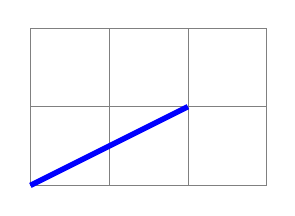
\begin{tikzpicture}[blue,line width=2pt]
\draw[help lines] (0,0) grid (3,2); 
\draw  (0,0) -- (2,1) ; 
\end{tikzpicture}
&  
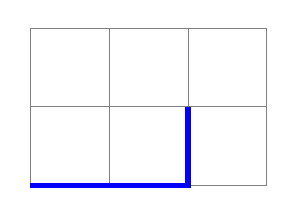
\begin{tikzpicture}[blue,line width=2pt]
\draw[help lines] (0,0) grid (3,2); 
\draw  (0,0) -| (2,1) ; 
\end{tikzpicture}
&
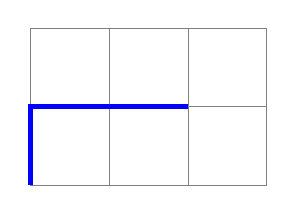
\begin{tikzpicture}[,blue,line width=2pt]
\draw[help lines] (0,0) grid (3,2); 
\draw  (0,0) |- (2,1) ; 
\end{tikzpicture}

\\ \hline 
\end{tabular} 
\end{center}
\bigskip
 
\noindent \begin{tabular}{|c|c|c|}\hline
 \multicolumn{3}{|c|}{\BS{draw} (0,2) . . \DDD{controls} (3,0)  .. (2,2); \RRR{ 14-3 }}
 \\  \hline 	 
  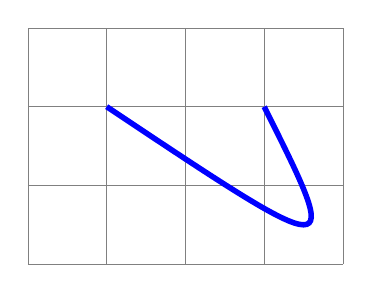
\begin{tikzpicture}[,blue,line width=2pt,fill=green]
  \draw[help lines] (-1,0) grid (3,3); 
\draw (0,2) .. controls (3,0)  .. (2,2);
  \end{tikzpicture}  
  &
  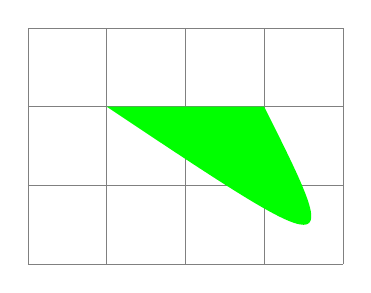
\begin{tikzpicture}[blue,line width=2pt,fill=green]
  \draw[help lines] (-1,0) grid (3,3); 
\fill (0,2) .. controls (3,0)  .. (2,2);
  \end{tikzpicture} 
  &
  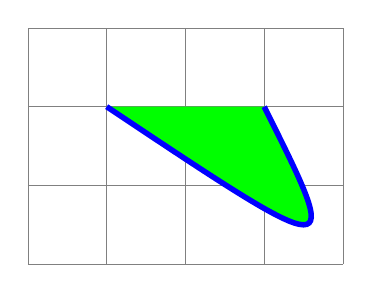
\begin{tikzpicture}[blue,line width=2pt,fill=green]
  \draw[help lines] (-1,0) grid (3,3); 
\filldraw (0,2) .. controls (3,0)  .. (2,2);
  \end{tikzpicture} 
  \\ \hline 
\BSS{draw} 
&  
\BSS{fill} 
&  
\BSS{filldraw} 
\\ \hline
 \end{tabular}
 
 
 \bigskip

\noindent
 \begin{tabular}{|c|c|c|}\hline
 \multicolumn{3}{|c|}{\BS{draw} (0,2) . . \DDD{controls} (3,0) \DDD{and} (-1,0) .. (2,2); \RRR{14-3}}
 \\  \hline 	 
  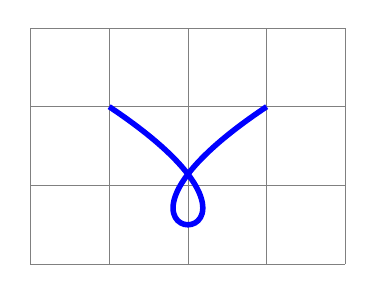
\begin{tikzpicture}[blue,line width=2pt,fill=green]
  \draw[help lines] (-1,0) grid (3,3); 
\draw (0,2) .. controls (3,0) and (-1,0) .. (2,2);
  \end{tikzpicture}  
  &
  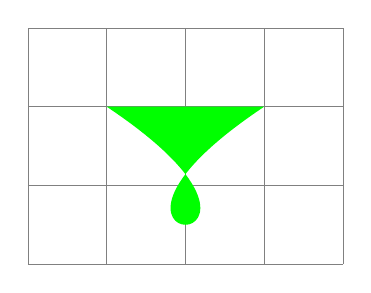
\begin{tikzpicture}[blue,line width=2pt,fill=green]
  \draw[help lines] (-1,0) grid (3,3); 
\fill (0,2) .. controls (3,0) and (-1,0) .. (2,2);
  \end{tikzpicture} 
  &
  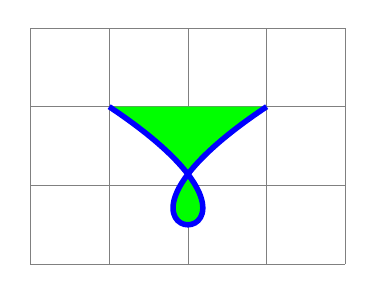
\begin{tikzpicture}[blue,line width=2pt,fill=green]
  \draw[help lines] (-1,0) grid (3,3); 
\filldraw (0,2) .. controls (3,0) and (-1,0) .. (2,2);
  \end{tikzpicture} 
  \\ \hline 
\BSS{draw} 
&  
\BSS{fill} 
&  
\BSS{filldraw} 
\\ \hline
 \end{tabular}


%--------------------------------------------------

\bigskip
\noindent \begin{tabular}{|c|c|c|} \hline
\multicolumn{3}{|c|}{\BS{draw} (0,0) \DDD{rectangle} (3,2); \RRR{14-4} }\\ 
\hline 
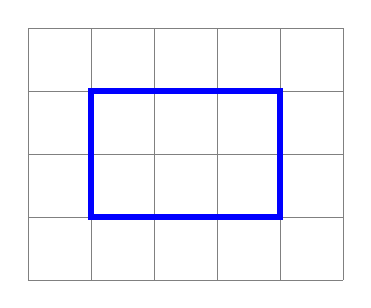
\begin{tikzpicture}[scale=.8,blue,line width=2pt]
\draw[help lines] (-1,-1) grid (4,3); 
\draw (0,0) rectangle (3,2);
\end{tikzpicture}
&  
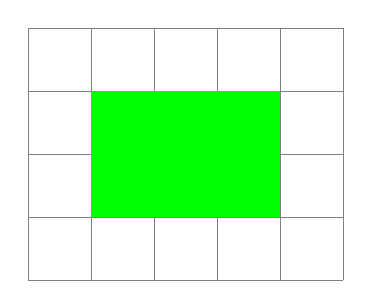
\begin{tikzpicture}[scale=.8,blue,line width=2pt,fill=green]
\draw[help lines] (-1,-1) grid (4,3); 
\fill (0,0) rectangle (3,2);
\end{tikzpicture}
&  
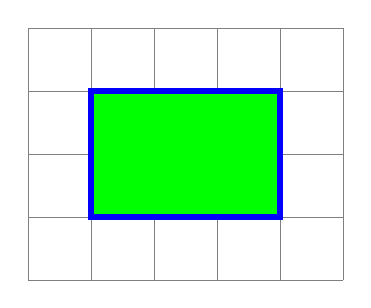
\begin{tikzpicture}[scale=.8,blue,line width=2pt,fill=green]
\draw[help lines] (-1,-1) grid (4,3); 
\filldraw (0,0) rectangle (3,2);
\end{tikzpicture}
\\ \hline  
\BSS{draw} 
&  
\BSS{fill} 
&  
\BSS{filldraw} 
\\ \hline

\end{tabular} 
 %-----------------------------------------------------
 
 \bigskip
  
\noindent \begin{tabular}{|c|c|c|}\hline
 \multicolumn{3}{|c|}{\BS{draw} (1,1) \DDD{circle} (1); \RRR{14-6}}\\ 
 \hline 
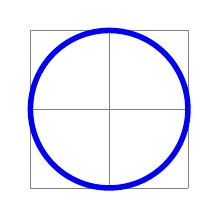
\begin{tikzpicture}[blue,line width=2pt,fill=green]
\draw[help lines] (0,0) grid (2,2); 
\draw (1,1) circle (1);	
\end{tikzpicture}  
&
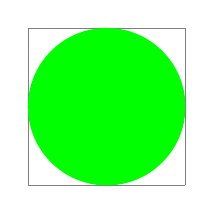
\begin{tikzpicture}[blue,line width=2pt,fill=green]
\draw[help lines] (0,0) grid (2,2); 
\fill (1,1) circle (1);	
\end{tikzpicture} 
&
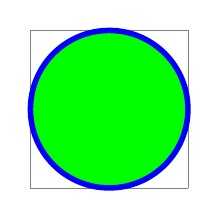
\begin{tikzpicture}[,blue,line width=2pt,fill=green]
\draw[help lines] (0,0) grid (2,2); 
\filldraw (1,1) circle (1);	
\end{tikzpicture} 
  \\ \hline 
  \BS{draw} 
  &  
  \BS{fill} 
  &  
  \BS{filldraw} 
  \\ \hline
\end{tabular} 


 %-----------------------------------------------------
 \bigskip
  
\noindent \begin{tabular}{|c|c|c|}\hline
 \multicolumn{2}{|c|}{\BS{draw} (1,1) \DDD{circle} [\RDD{radius}=1cm]; } & 
 \BS{draw} (1,1)\DDD{ellipse} [\RDD{x radius}=2cm,\RDD{y radius}=1cm]
\\  \hline 
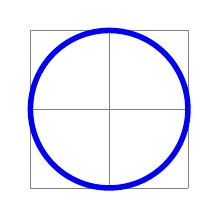
\begin{tikzpicture}[blue,line width=2pt,fill=green]
\draw[help lines] (0,0) grid (2,2); 
  \draw (1,1) circle [radius=1cm] ;	
  \end{tikzpicture}  
  &
  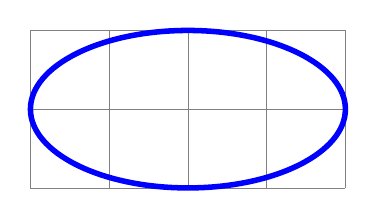
\begin{tikzpicture}[,blue,line width=2pt,fill=green]
  \draw[help lines] (-1,0) grid (3,2); 
  \draw (1,1) circle[x radius=2cm,y radius=1cm] ;	
  \end{tikzpicture} 
  &
   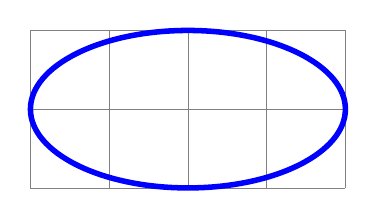
\begin{tikzpicture}[blue,line width=2pt,fill=green]
   \draw[help lines] (-1,0) grid (3,2); 
 \draw  (1,1) ellipse [x radius=2cm,y radius=1cm];	
   \end{tikzpicture}  
  \\ \hline 
\RDD{radius}=1cm & \RDD{x radius}=2cm,\RDD{y radius}=1cm
  \\ \hline 
\end{tabular} 
 %-----------------------------------------------------
 \bigskip
  
\noindent \begin{tabular}{|c|c|}\hline
\BS{draw}  (1,1) circle {\color{red}(2 and 1)}; & \BS{draw}  (1,1) ellipse {\color{red}(2 and 1)};  
 \\ \hline 	
  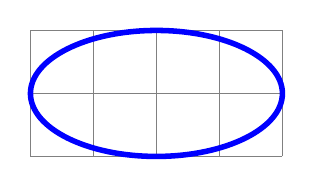
\begin{tikzpicture}[scale=.8,blue,line width=2pt,fill=green]
 \draw[help lines] (-1,0) grid (3,2); 
\draw  (1,1) circle(2 and 1);
  \end{tikzpicture}  
  &	
  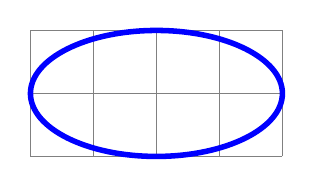
\begin{tikzpicture}[scale=.8,blue,line width=2pt,fill=green]
 \draw[help lines] (-1,0) grid (3,2); 
\draw  (1,1) ellipse (2 and 1);
  \end{tikzpicture}  
\\ \hline 
  \end{tabular}

\bigskip

\noindent \begin{tabular}{|c|c|c|}\hline 
\multicolumn{3}{|c|}{\BS{draw} (-2,0) \DDD{arc} (180:-45:2); \RRR{14-7} }\\ 
\hline  	
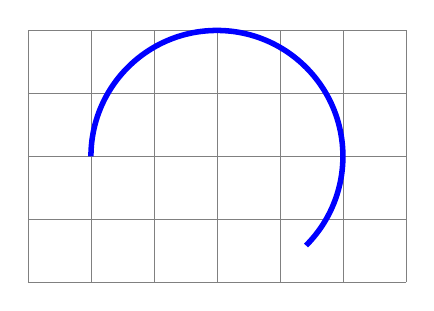
\begin{tikzpicture}[scale=.8,blue,line width=2pt,fill=green]
\draw[help lines] (-3,-2) grid (3,2);
\draw (-2,0) arc (180:-45:2); 	
\end{tikzpicture} 
&
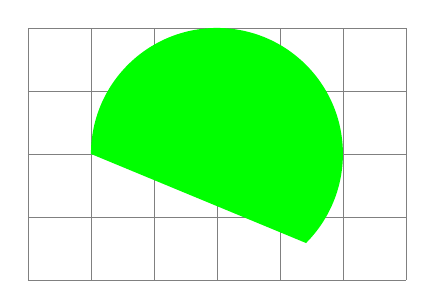
\begin{tikzpicture}[scale=.8,blue,line width=2pt,fill=green]
\draw[help lines] (-3,-2) grid (3,2);
\fill (-2,0) arc (180:-45:2); 
\end{tikzpicture} 
&
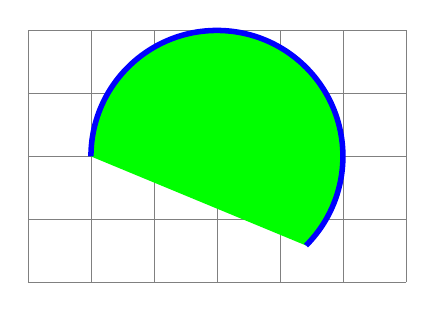
\begin{tikzpicture}[scale=.8,blue,line width=2pt,fill=green]
\draw[help lines] (-3,-2) grid (3,2);
\filldraw (-2,0) arc (180:-45:2); 	
\end{tikzpicture}
\\ \hline 
\BS{draw} 
&  
\BS{fill} 
&  
\BS{filldraw} 
\\ \hline
 \end{tabular} 
 \bigskip
 
\noindent \begin{tabular}{|c|c||c|}  \hline 
\multicolumn{2}{|c||}{\BS{draw} (-2,0) arc [\RDD{start angle}=180, \RDD{end angle}=-45,\RDD{radius}=1] }
& \BS{draw} (-2,0) \RDD{ arc (180:-45:2 and 1)}
\\ \hline  	
  
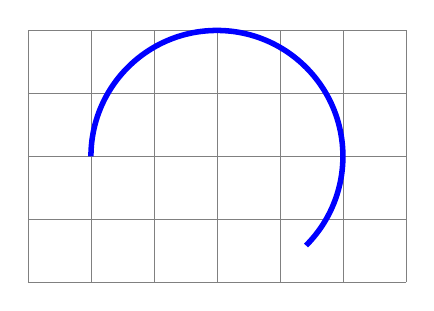
\begin{tikzpicture}[scale=.8,blue,line width=2pt,fill=green]
\draw[help lines] (-3,-2) grid (3,2);
\draw (-2,0) arc [start angle=180, end angle=-45,radius=2]; 	
\end{tikzpicture}
 &  
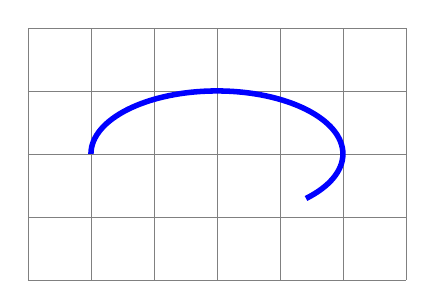
\begin{tikzpicture}[scale=.8,blue,line width=2pt,fill=green]
\draw[help lines] (-3,-2) grid (3,2);
\draw (-2,0) arc [start angle=180, end angle=-45,x radius=2,y radius=1]; 	
\end{tikzpicture}
&
  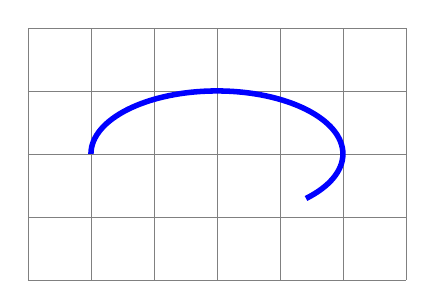
\begin{tikzpicture}[scale=.8,blue,line width=2pt,fill=green]
\draw[help lines] (-3,-2) grid (3,2);
\draw (-2,0)  arc (180:-45:2 and 1);
%\draw [dotted,line width=1pt] (0,0) ellipse [x radius=2cm,y radius=1cm];   
\end{tikzpicture}
 \\  \hline 
 \RDD{radius}=1 & \RDD{x radius}=1,\RDD{y radius}=.5 & \\ 
 \hline 
 \end{tabular} 

\bigskip
 
\noindent \begin{tabular}{|c|c|c|}\hline  
 \multicolumn{3}{|c|}{\BS{draw} (0,0) \DDD{parabola} (3,2);   \RRR{14-9} }
 \\ \hline 	
   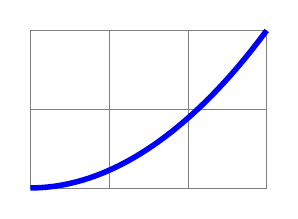
\begin{tikzpicture}[blue,line width=2pt,fill=green]
   \draw[help lines] (0,0) grid (3,2); 
 \draw (0,0) parabola (3,2); 
   \end{tikzpicture}  
   &
   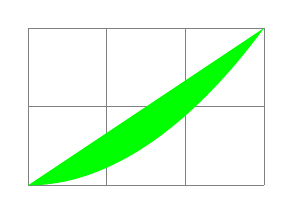
\begin{tikzpicture}[blue,line width=2pt,fill=green]
   \draw[help lines] (0,0) grid (3,2); 
 \fill (0,0) parabola (3,2); 
   \end{tikzpicture} 
   &
   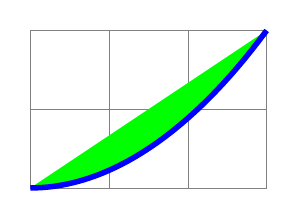
\begin{tikzpicture}[blue,line width=2pt,fill=green]
   \draw[help lines] (0,0) grid (3,2); 
 \filldraw (0,0) parabola (3,2); 
   \end{tikzpicture} 
   \\ \hline 
\BS{draw} 
&  
\BS{fill} 
&  
\BS{filldraw} 
\\ \hline
   \end{tabular} ------
 
\noindent \begin{tabular}{|c|c|} \hline  
 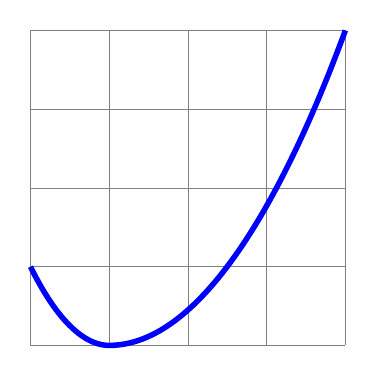
\begin{tikzpicture}[blue,line width=2pt,fill=green]
 \draw[help lines] (0,0) grid (4,4); 
 \draw(0,1) parabola bend (1,0) (4,4); 
  \end{tikzpicture}
 & 
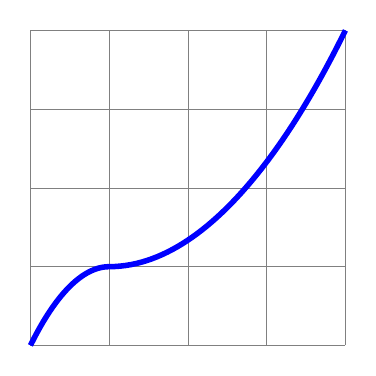
\begin{tikzpicture}[blue,line width=2pt,fill=green]
\draw[help lines] (0,0) grid (4,4); 
\draw (0,0) parabola[bend pos=0.25] (4,4);
 \end{tikzpicture} \\ 
 \hline 
  \BS{draw}(0,1) parabola \RDD{bend} (1,0) (4,4); & 
  \BS{draw}(0,0) parabola[\RDD{bend pos}=0.25] (4,4); 
  \\  \hline 
 \end{tabular} 
\bigskip

\noindent \begin{tabular}{|c|c|c|} \hline 
 \BS{draw}(0,1) parabola [\RDD{parabola height}=2cm] (3,0);  & \multicolumn{2}{|c|}{\BS{draw}(0,0) parabola[\RDD{bend at start}] (3,2);}\\ 
 \hline 
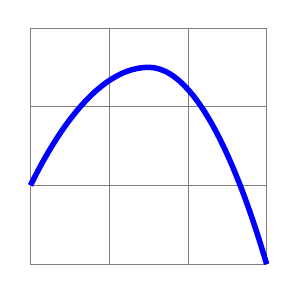
\begin{tikzpicture}[blue,line width=2pt,fill=green]
\draw[help lines] (0,0) grid (3,3); 
\draw (0,1) parabola[parabola height=2cm] (3,0);
 \end{tikzpicture}  & 
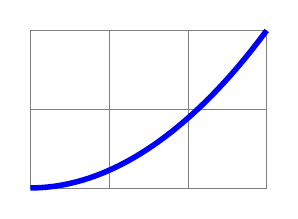
\begin{tikzpicture}[blue,line width=2pt,fill=green]
\draw[help lines] (0,0) grid (3,2); 
\draw (0,0) parabola[bend at start] (3,2);
 \end{tikzpicture}
&  
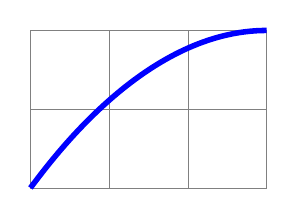
\begin{tikzpicture}[blue,line width=2pt,fill=green]
\draw[help lines] (0,0) grid (3,2); 
\draw (0,0) parabola[bend at end] (3,2);
 \end{tikzpicture}
\\ \hline &[\RDD{bend at start}]  & [\RDD{bend at end}] \\ 
\hline 
\end{tabular}  

\bigskip
 
\noindent \begin{tabular}{|c|c|c|}\hline 
 \multicolumn{3}{|c|}{\BS{draw} (0,0) \DDD{sin}  (1.57,2);  \RRR{14-10} }\\ 
 \hline 	
  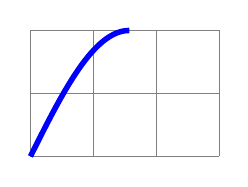
\begin{tikzpicture}[scale=.8,blue,line width=2pt,fill=green]
  \draw[help lines] (0,0) grid (3,2); 
\draw  (0,0) sin (1.57,2); 
  \end{tikzpicture}  
  &
  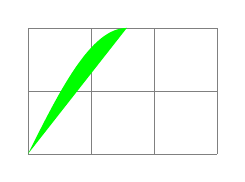
\begin{tikzpicture}[scale=.8,blue,line width=2pt,fill=green]
  \draw[help lines] (0,0) grid (3,2); 
\fill  (0,0) sin (1.57,2); 
  \end{tikzpicture} 
  &
  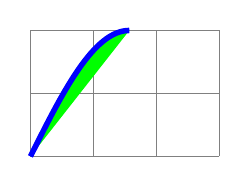
\begin{tikzpicture}[scale=.8,blue,line width=2pt,fill=green]
  \draw[help lines] (0,0) grid (3,2); 
\filldraw (0,0) sin (1.57,2); 
  \end{tikzpicture} 
  \\ \hline 
 \BS{draw} 
 &  
 \BS{fill} 
 &  
 \BS{filldraw} 
 \\ \hline 	


  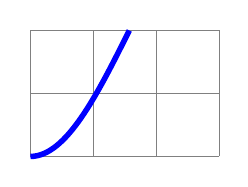
\begin{tikzpicture}[scale=.8,blue,line width=2pt,fill=green]
  \draw[help lines] (0,0) grid (3,2); 
\draw  (0,0) cos (1.57,2); 
  \end{tikzpicture}  
  &
  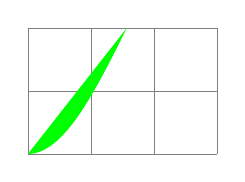
\begin{tikzpicture}[scale=.8,blue,line width=2pt,fill=green]
  \draw[help lines] (0,0) grid (3,2); 
\fill  (0,0) cos (1.57,2); 
  \end{tikzpicture} 
  &
  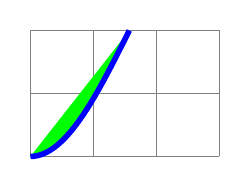
\begin{tikzpicture}[scale=.8,blue,line width=2pt,fill=green]
  \draw[help lines] (0,0) grid (3,2); 
\filldraw (0,0) cos (1.57,2); 
  \end{tikzpicture} 
  \\ \hline 
\multicolumn{3}{|c|}{\BS{draw} (0,0) \DDD{cos}  (1.57,2);  }\\ 
\hline 	 	
 \end{tabular} 
  %----------------------------------------------------
\bigskip
  
\begin{center}
\RRR{14-13}
\end{center}
  
\noindent \begin{tabular}{|c|c|c|} \hline  
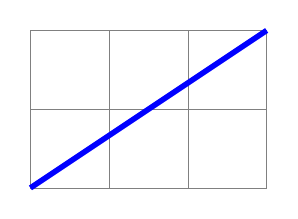
\begin{tikzpicture}[blue,line width=2pt,fill=green]
\draw[help lines] (0,0) grid (3,2); 
\draw  (0,0) to (3,2); 
\end{tikzpicture} 
&  
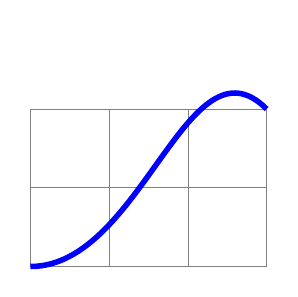
\begin{tikzpicture}[blue,line width=2pt,fill=green]
\draw[help lines] (0,0) grid (3,2); 
\draw[out=0]  (0,0) to  (3,2); 
\end{tikzpicture}
&  
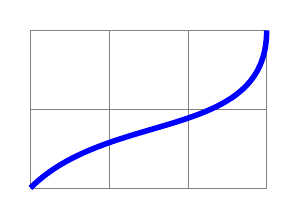
\begin{tikzpicture}[blue,line width=2pt,fill=green]
\draw[help lines] (0,0) grid (3,2); 
\draw[in=-90]  (0,0) to  (3,2); 
\end{tikzpicture}
\\ \hline  
\BS{draw}  (0,0) \DDD{to} (3,2);& \BS{draw}[\RDD{out}=0]  (0,0) to (3,2); & \BS{draw} [\RDD{in}=-90]  (0,0) to (3,2); 
\\  \hline 
\multicolumn{3}{|c|}{\TFRGB{voir}{see} section \ref{liaisons} page \pageref{liaisons}  }\\ 
\hline

\end{tabular} 

%----------------------------------------------
\bigskip



\noindent \begin{tabular}{|c|c|c|} \hline
\multicolumn{2}{|c|}{ \bf{\TFRGB{Dessin avec plot}{Drawing with plot} }}
\RRR{14-12} \RRR{22}
\\ \hline

\TFRGB{une liste de coordonnées}{list of coordinates} & \TFRGB{un fichier de coordonnées}{file of coordinates} & \TFRGB{une équation mathématique}{mathematical equation}
     \\ \hline
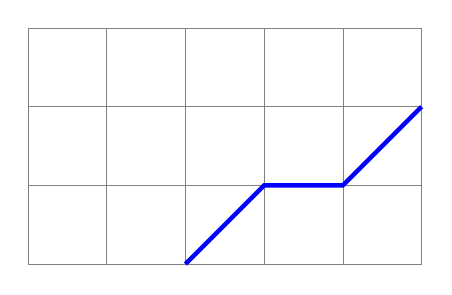
\begin{tikzpicture}[blue,line width=2pt,fill=green] 
\draw[help lines] (0,0) grid (5,3); 
\draw[blue,ultra thick] plot coordinates {(2,0) (3,1) (4,1) (5,2)};
\end{tikzpicture}
   &

\begin{tikzpicture}[blue,line width=2pt,fill=green] 
\draw[help lines] (0,0) grid (3,3);
\draw[blue,ultra thick] plot file {table.dat};
\end{tikzpicture}
   &
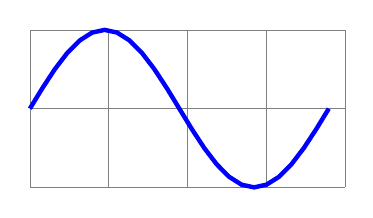
\begin{tikzpicture}[blue,line width=2pt,fill=green] 
\draw[help lines] (0,-1) grid (4,1); \draw[blue,domain=0:360,x=0.3,ultra thick] plot (\x,{sin(\x)});
 \end{tikzpicture}
  \\ \hline 
 plot coordinates  	&  plot file \AC{table.dat} &  plot (\BS{x},\AC{sin(\BS{x})}) \\
  \AC{(2,0) (3,1) (4,1) (5,2)} &&
  \\ \hline   
  \multicolumn{3}{|c|}{voir page \pageref{plot} }
 \\ \hline 

\end{tabular} 

 %---------------------------------------------------------
\newpage 

\SSCT{Chemin}{Path and edge}

\SbSSCT{Notion de Chemin}{Path}
\begin{center}
\RRR{14}
\end{center}

\noindent \begin{tabular}{|c|c|} \hline 
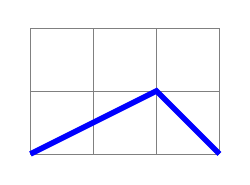
\begin{tikzpicture}[scale=.8,blue,line width=2pt]
\draw[help lines] (0,0) grid (3,2); 
\draw  (0,0) -- (2,1) -- (3,0) ; 
\end{tikzpicture}
& 
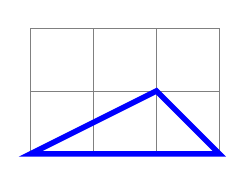
\begin{tikzpicture}[scale=.8,blue,line width=2pt]
\draw[help lines] (0,0) grid (3,2); 
\draw  (0,0) -- (2,1) -- (3,0) -- cycle ; 
\end{tikzpicture}
\\ \hline
\BS{draw}  (0,0) - - (2,1) - - (3,0) ; 

& 
\BS{draw}  (0,0) -  - (2,1) -  - (3,0) -  - \RDD{cycle} ; 
\\ \hline 
\end{tabular} 

\bigskip
\noindent \begin{tabular}{|c|c|} \hline 
 \multicolumn{2}{|c|}{  \BS{draw} (0,0) - - (2,1) - - (3,3)  arc (135:-20:1)   .. controls (6,0) and (4,0) }\\
 \multicolumn{2}{|c|}{  .. (5,2) sin (6.57,0) cos (7.57,2) ;}
 \\ \hline
 
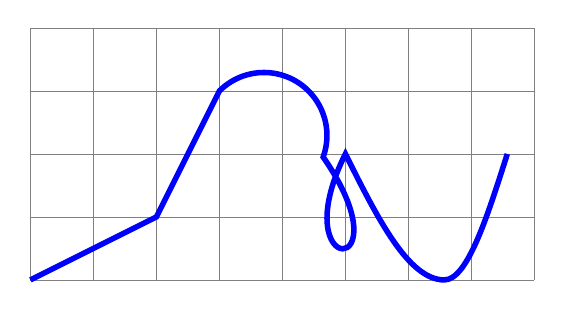
\begin{tikzpicture}[scale=.8,blue,line width=2pt]
\draw[help lines] (0,0) grid (8,4); 
\draw  (0,0) -- (2,1) -- (3,3)  arc (135:-20:1)   .. controls (6,0) and (4,0) .. (5,2) sin (6.57,0) cos (7.57,2) ;
\end{tikzpicture}
&  
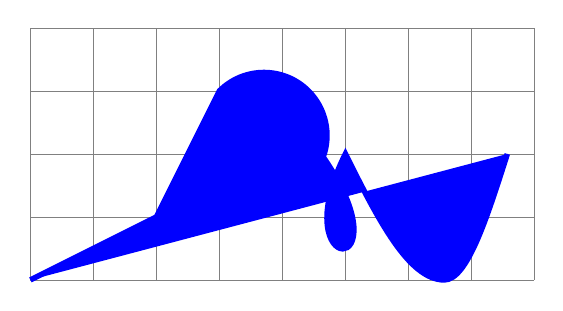
\begin{tikzpicture}[scale=.8,blue,line width=2pt]
\draw[help lines] (0,0) grid (8,4); 
\filldraw  (0,0) -- (2,1) -- (3,3)  arc (135:-20:1)   .. controls (6,0) and (4,0) .. (5,2) sin (6.57,0) cos (7.57,2) ;
\end{tikzpicture}
\\ \hline 
\BS{draw} & \BS{filldraw}
\\ \hline  
\end{tabular} 





\bigskip 
\begin{center}
\RRR{14-5 } 
\end{center}

  
\noindent \begin{tabular}{|c|c|} \hline 
\begin{tikzpicture}[scale=.8,blue,line width=4mm]
\draw[help lines] (0,0) grid (3,2); 
\draw [rounded corners] (0,0) -- (2,1) -- (3,0) ; 
\end{tikzpicture}
& 
\begin{tikzpicture}[scale=.8,blue,line width=4mm]
\draw[help lines] (0,0) grid (3,2); 
\draw [sharp corners] (0,0) -- (2,1) -- (3,0)  ; 
\end{tikzpicture}
\\ \hline
\BS{draw} [\RDD{rounded corners}] (0,0) -- (2,1) -- (3,0) ; 

& 
\BS{draw} [\RDD{sharp corners}] (0,0) -  - (2,1) -  - (3,0) ; 
\\ 
\hline 
\end{tabular} 

\bigskip
\noindent \begin{tabular}{|c|c|} \hline  
\begin{tikzpicture}[scale=.8,blue,baseline=0pt,line width=2pt]
\draw[help lines] (0,0) grid (2,2); 
\draw   (0,0) -- (1,1.732)  -- (2,0)  -- cycle ;  
\end{tikzpicture}
&  
\BS{draw} [\RDD{rounded corners}=0.5cm]   (0,0) - - (1,1.732) - - (2,0)  - - cycle ; 
\\ \hline  
\begin{tikzpicture}[scale=.8,blue,baseline=0pt,line width=2pt]
\draw[help lines] (0,0) grid (2,2); 
\draw   (0,0) -- (1,1.732) [rounded corners=0.5cm]  -- (2,0)  -- cycle ;  
\end{tikzpicture}
&  
\BS{draw}  (0,0) - - (1,1.732) [\RDD{rounded corners}=0.5cm]  - - (2,0)  - - cycle ;  
\\ \hline 
\begin{tikzpicture}[scale=.8,blue,baseline=0pt,line width=2pt]
\draw[help lines] (0,0) grid (2,2); 
\draw  (0,0) -- (1,1.732) -- (2,0)[rounded corners=0.5cm] -- cycle ; 
\end{tikzpicture}
&  
\BS{draw} (0,0) - - (1,1.732) - - (2,0)[\RDD{rounded corners}=0.5cm] - - cycle ;
\\ \hline 
\begin{tikzpicture}[scale=.8,blue,baseline=0pt,line width=2pt]
\draw[help lines] (0,0) grid (2,2); 
\draw [rounded corners=0.5cm]  (0,0) -- (1,1.732)[sharp corners] -- (2,0) -- cycle ; 
\end{tikzpicture}
&  
\BS{draw} [\RDD{rounded corners}=0.5cm]  (0,0) - - (1,1.732)[\RDD{sharp corners}] - - (2,0) - - cycle ; 
\\ \hline 

\end{tabular} 

\bigskip
\begin{center}
\RRR{14-2-2}
\end{center}


\noindent \begin{tabular}{|c|c|} \hline 
\begin{tikzpicture}[scale=.8,blue,line width=2pt]
\draw[help lines] (0,0) grid (3,2); 
\draw  (0,0) -- (2,1) -| cycle ; 
\end{tikzpicture}
& 
\begin{tikzpicture}[scale=.8,blue,line width=2pt]
\draw[help lines] (0,0) grid (3,2); 
\draw (0,0) -- (2,1) |- cycle  ; 
\end{tikzpicture}
\\ \hline
\BS{draw}  (0,0) - - (2,1) \textbf{{\color{red}-|}} cycle  ; 
& 
\BS{draw} (0,0) - - (2,1) \textbf{{\color{red}|-}} cycle  ; 
\\ 
\hline 
\end{tabular} 

\bigskip

\noindent \begin{tabular}{|c|} \hline  
\BS{tikz} [{\color{red} c/.style}=\AC{\RDD{insert path}=\AC{circle[radius=3pt]}}] \\
\BS{draw}(0,0){\color{red}[c]} -- (1,2){\color{red}[c]} -- (3,1) {\color{red}[c]};
\\ \hline  
\begin{tikzpicture}[c/.style={insert path={circle[radius=3pt]}}]
\draw[help lines] (0,0) grid (4,3); 
\draw(0,0)[c] -- (1,2)[c]  -- (3,1) [c];
\end{tikzpicture}
\\ \hline 
\end{tabular} 


%TODO 2 commandes pour expert à voir plus tard

%\tikz \draw node [append after command={(xxx)--(1,1)},draw] (xxx){noeud};
%
%\tikz \fill  [append after command={[blue](0,0) rectangle (2,2)},draw] [red](1,1) rectangle (3,3);
%
%\tikz \draw node [prefix after command={(foo)--(1,1)},draw] (foo){foo};
%
%\tikz \fill  [prefix after command={[blue](0,0) rectangle (2,2)},draw] [red](1,1) rectangle (3,3);
\bigskip

\bf{\TFRGB{Coupure de chemin}{Path interrupted}} \RRR{14-1}

\bigskip

\noindent \begin{tabular}{|c|} \hline 
\BS{draw} (0.5,0.5) - -(2.5,0.5)   (0.5,1.5) - -(2.5,1.5);
\\ \hline 
\begin{tikzpicture}[blue,line width=2pt]
\draw[help lines] (0,0) grid (3,2); 
\draw (0.5,0.5) - -(2.5,0.5)   (0.5,1.5) - -(2.5,1.5);
\end{tikzpicture}
\\ \hline 
\end{tabular} 

\bigskip

\noindent \begin{tabular}{|c|} \hline  
\BS{draw} (0,0) - - (0,1) - - (1,1) (2,0) - - (2,1)
- - (3,1) - - (\BDD{current subpath start}); \\
\BS{fill}[red]  (\BDD{current subpath start}) circle (3pt);
\\ \hline 
\begin{tikzpicture}[blue,baseline=0pt,line width=2pt]
\draw[help lines] (0,0) grid (4,2); 
\draw (0,0) -- (0,1) -- (1,1) (2,0) -- (2,1)
-- (3,1) -- (current subpath start);
\fill[red]  (current subpath start) circle (3pt);
\end{tikzpicture}
\\ \hline 
\end{tabular} 

\SbSSCT{Chemins dans un chemin}{Pathes in a path : edge}

\begin{center}
 \RRR{17-12} 
\end{center}
 
 \bigskip
 
\begin{tabular}{|c|}  \hline  
\BS{draw} (0,0) - - (2,1) \RDD{edge}[dotted] (3,0) \RDD{edge}[red] (3,2)  - -(1,2) - -  (0,1) ;

\\ \hline  
\begin{tikzpicture}[blue,baseline=0pt,line width=2pt]
\draw[help lines] (0,0) grid (3,2);
\draw (0,0) - - (2,1) edge[dotted] (3,0) edge[red] (3,2)  --(1,2) --  (0,1) ;
\end{tikzpicture}
\\ \hline 
\end{tabular}  

 \bigskip
 
\begin{tabular}{|c|}  \hline  
\BS{draw} (0,0) - - (2,1) \RDD{edge}([red,\BDD{to path=\AC{parabola (3,0)} }] () \\
\RDD{edge}[red,\BDD{to path=\AC{arc(-90 : 90 : 0.5)}}] ()   - -(1,2) - -  (0,1) ;

\\ \hline 
\begin{tikzpicture}[blue,baseline=0pt,line width=2pt]
\draw[help lines] (0,0) grid (3,2);
\draw (0,0) - - (2,1) edge[red,to path={parabola (3,0)}] ()  edge[red,to path={arc(-90 :90 :.5)}] ()   --(1,2) --  (0,1) ;
\end{tikzpicture}
\\ \hline 
\end{tabular} 